\section{Mean Temperature Each Day of the Year}
The purpose of this exercise, referred to as "3.2 The temperature for every day of the year" in the project instructions, is to create a program which returns a plot of the mean temperature for each day of a given year. The plot should also contain error bars representing the standard deviation of the corresponding mean values.

For this program a data set of temperature measurements in Lund was used. This data set ranges from 1961 to 2015. My objective was to write a program which could produce the desired plot for any of these years.

\subsection{Code}
The code is written such that it should be able to run in ROOT since that is where we want to produce the plots.

Firstly the SMHI data set file, containing lines of text and superfluous data, had to be trimmed down to just provide data interesting to this exercise. This was done using a bash script. This bash script trims down the data so that descriptive lines of text is excluded using the \textbf{cut}-command. Every line of data has a quality marker, and using the \textbf{grep}-command the unapproved lines of data could be removed. This altered data is then saved to a new textfile. This bash script is called with the \textbf{system()}-function and can therefore be executed within the main program.

This textfile is read using a \textbf{while} loop, where the \textbf{getline()} function is used to extract strings of information. These strings are later converted into integers/doubles. Since this loop reads the entire file, an input variable specifying the desired year that is to be plotted is used to create an \textbf{if}-statement where the mean temperature values for each day and their associated standard deviation values are determined and stored in a histogram previously defined. This histogram has 366 bins corresponding to the days of the year, each bin is therefore filled with only one value. This way only values for each day of a specific year is plotted.

Exiting the \textbf{while} loop the file is closed and using the \textbf{Draw()} function the filled histogram is drawn with error bars.

\subsection{Results}
Since the purpose of the exercise was to simply plot the mean temperatures for each day with error bars representing the standard deviation no further analysis of the data was performed. The written program takes a given year and plots the temperatures for that year. The program does not take leap years into account, on non-leap years the 366th bin will be empty. This is something that could be done if we would perfect the code further. Figure \ref{1961}, \ref{1980}, \ref{2000}, \ref{2011} show plots for the years 1961, 1980, 2000 and 2011 respectively. Observe that 1980 and 2000 were leap years.

\begin{figure}
    \centering
    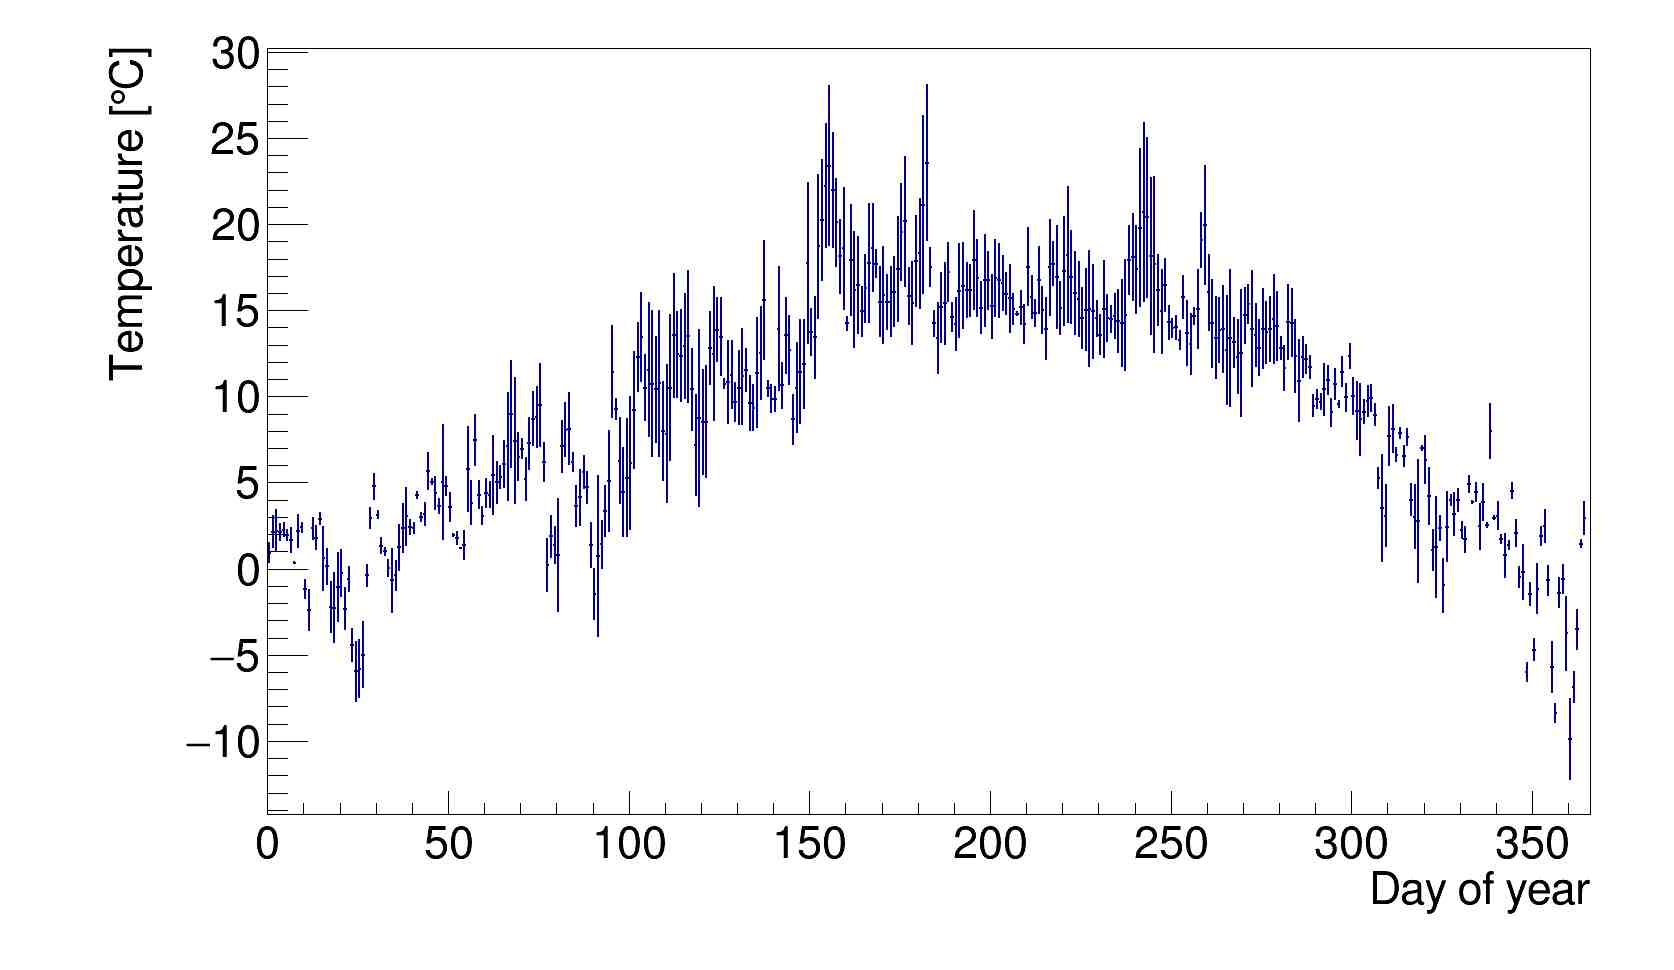
\includegraphics[width=14cm]{eachday1961.jpg}
    \caption{Mean temperatures for each day of 1961.}
    \label{1961}
\end{figure}

\begin{figure}
    \centering
    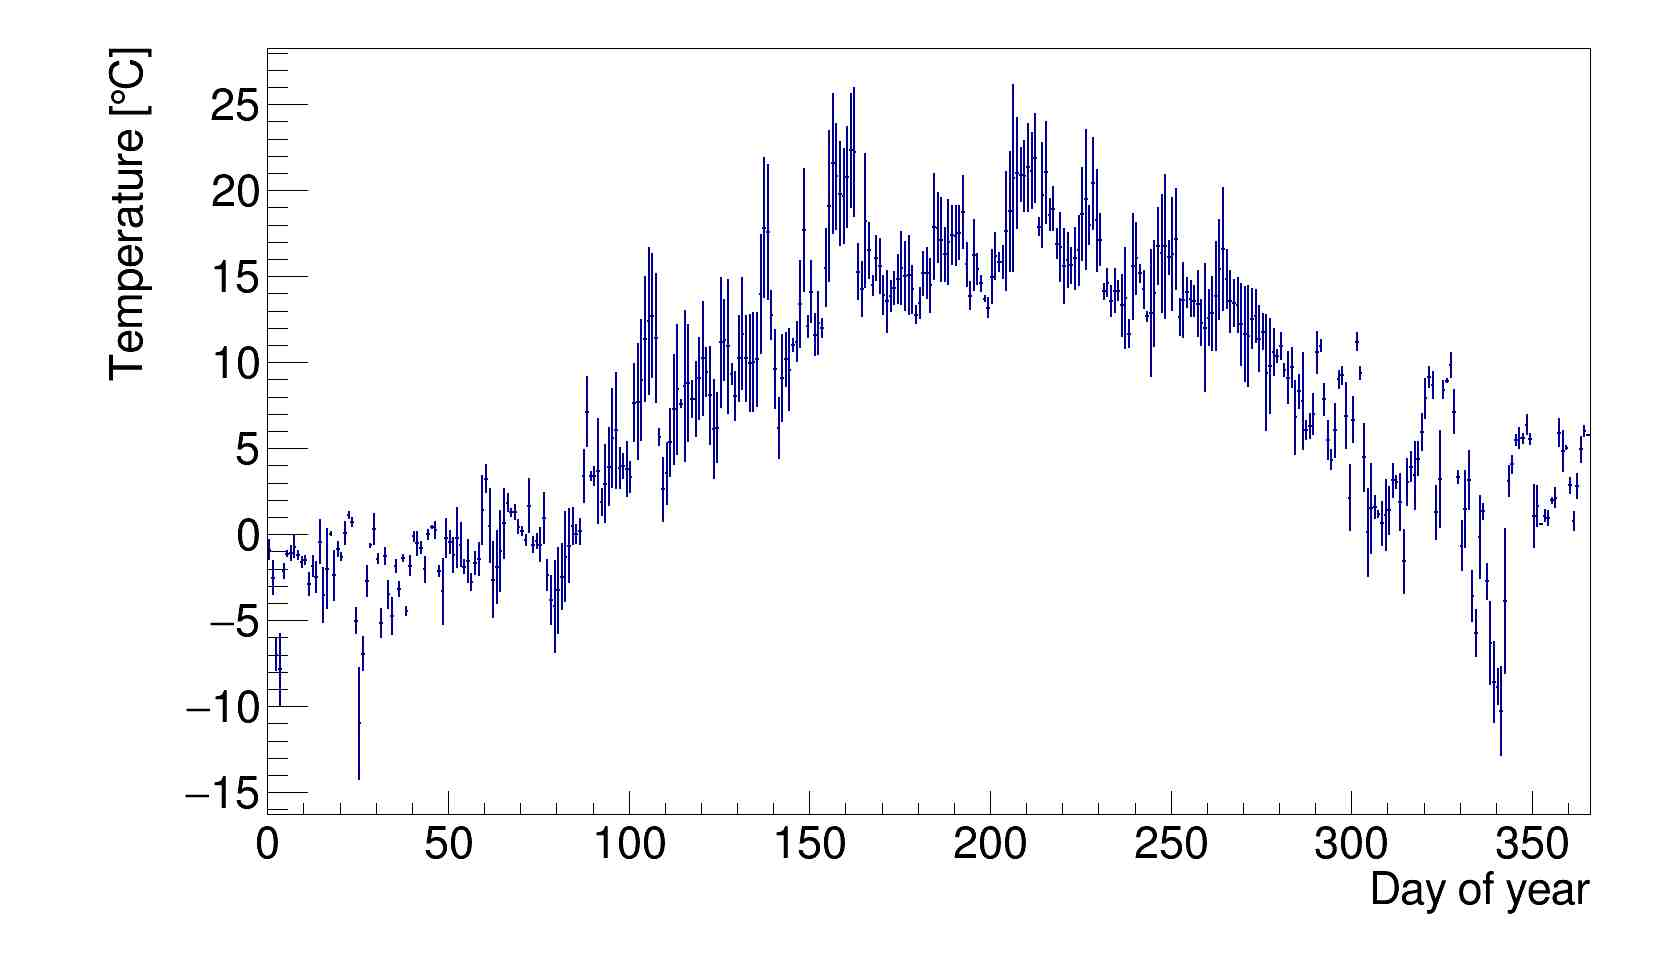
\includegraphics[width=14cm]{eachday1980.jpg}
    \caption{Mean temperatures for each day of 1980.}
    \label{1980}
\end{figure}

\begin{figure}
    \centering
    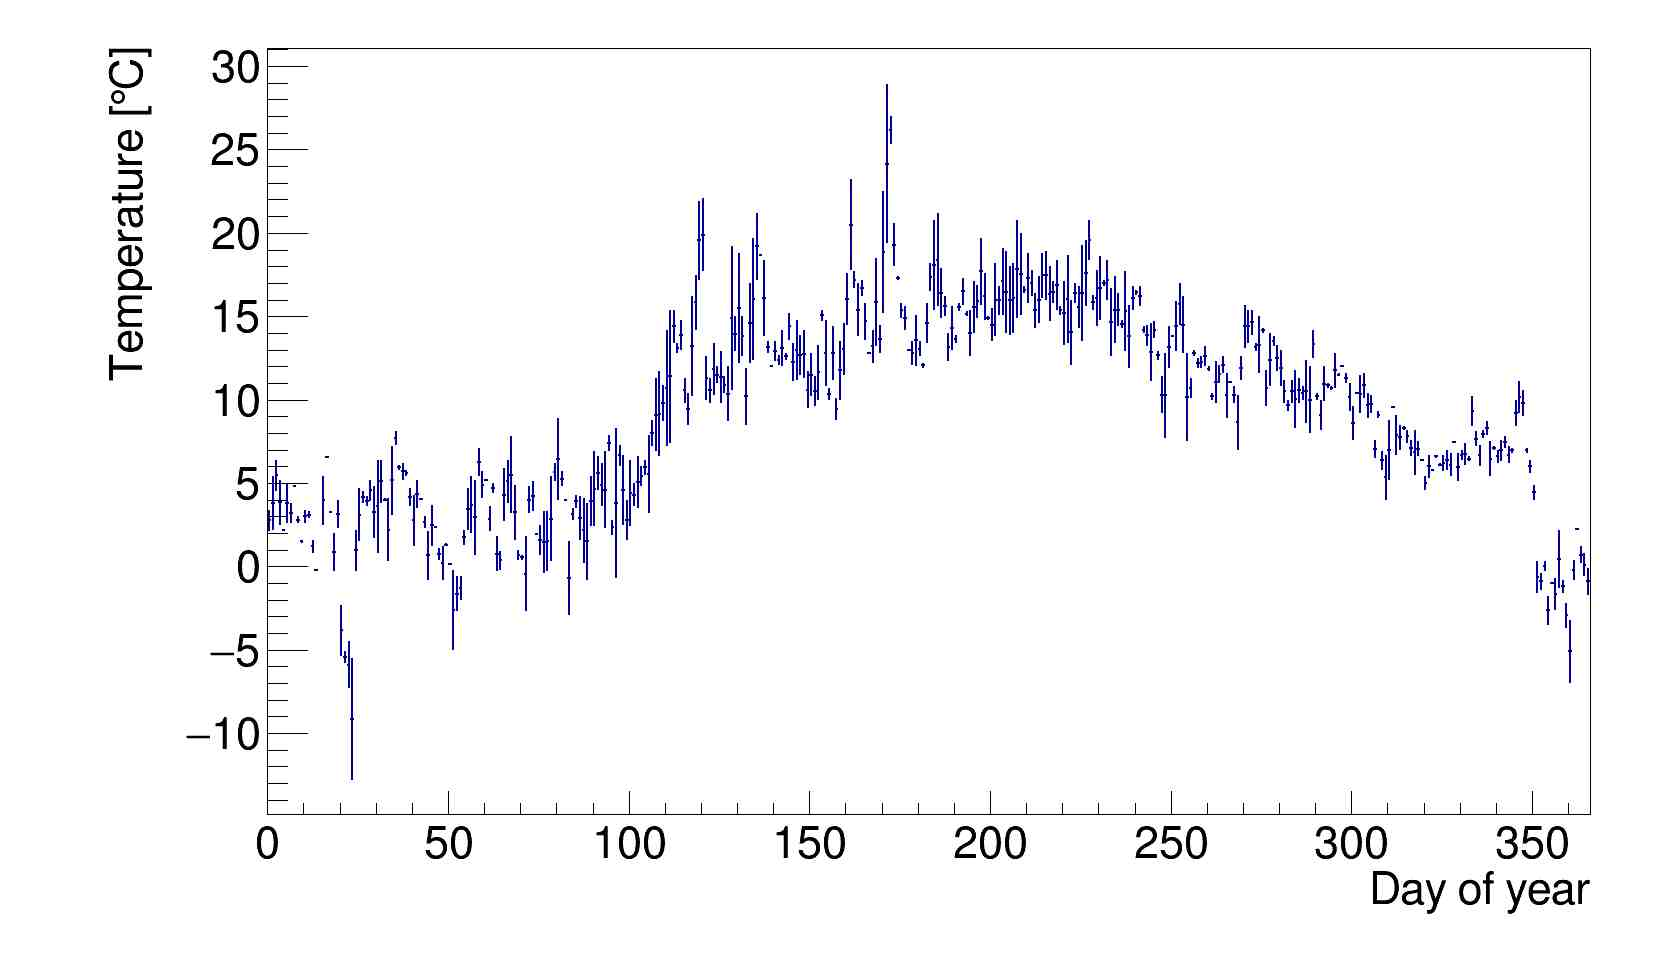
\includegraphics[width=14cm]{eachday2000.jpg}
    \caption{Mean temperatures for each day of 2000.}
    \label{2000}
\end{figure}

\begin{figure}
    \centering
    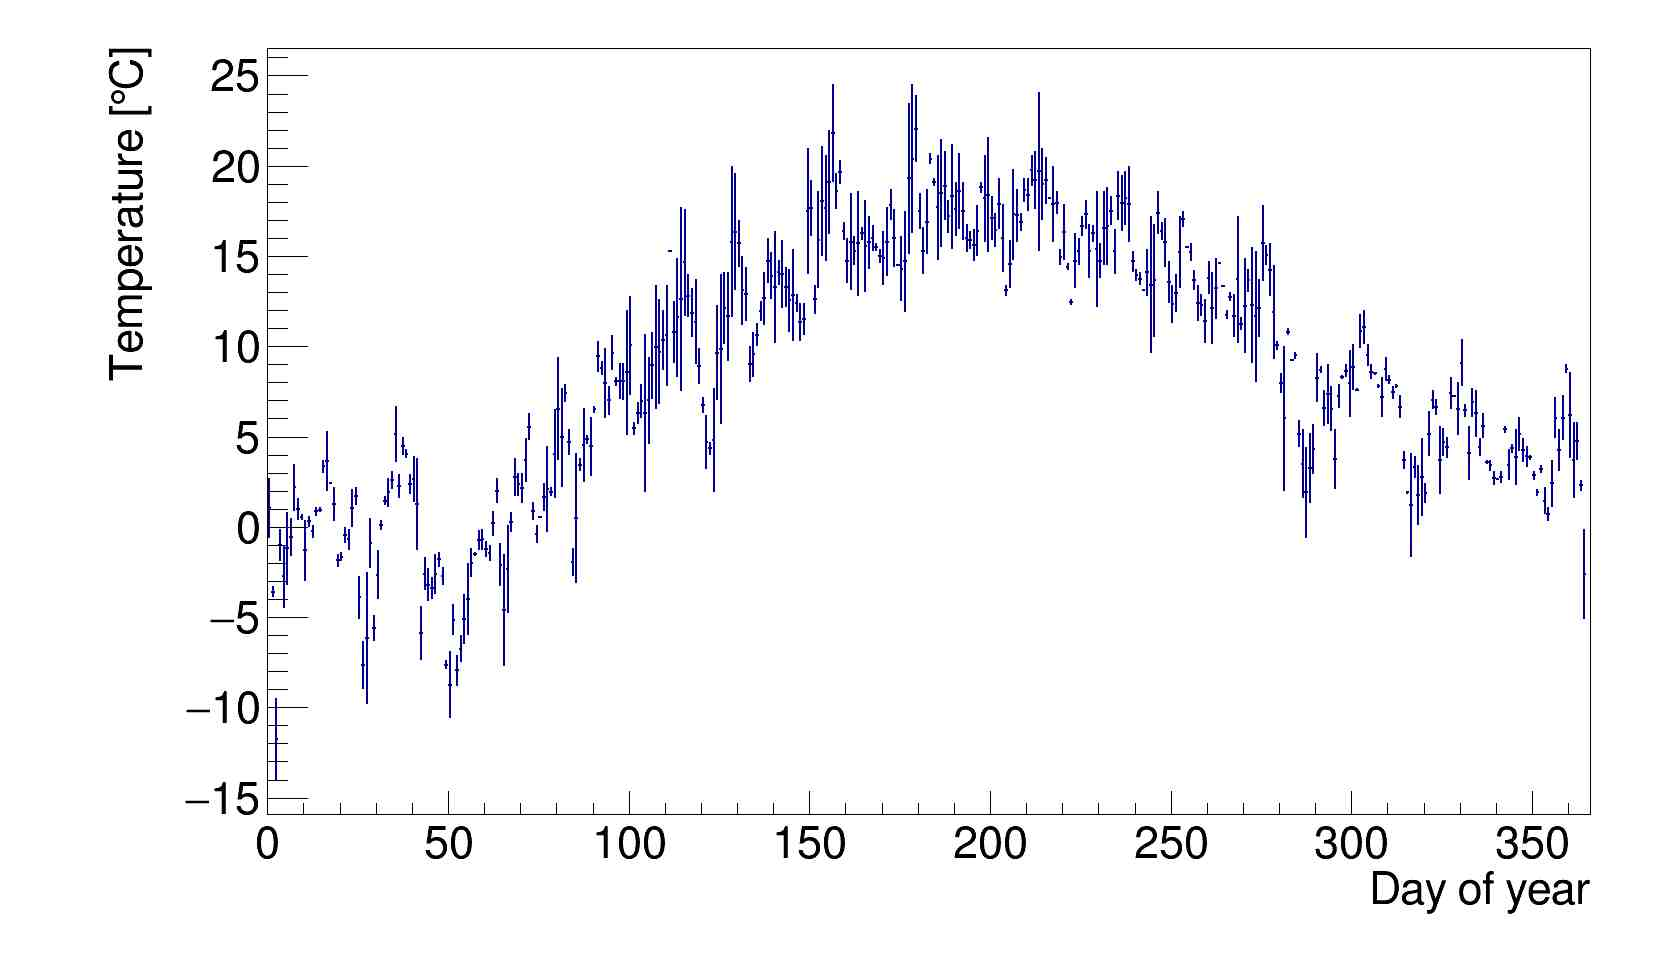
\includegraphics[width=14cm]{eachday2011.jpg}
    \caption{Mean temperatures for each day of 2011.}
    \label{2011}
\end{figure}
